\documentclass[pdf]{beamer}

%Subhi's styles
%\usecolortheme{whale}
%\usecolortheme{orchid}
%\useinnertheme[shadow]{rounded}
%\useoutertheme{infolines}

%%Alternative
%\usetheme{Warsaw}

\usetheme{Madrid}

\usepackage{pgfpages}
%\setbeameroption{show notes on second screen}
%\setbeameroption{show notes}


\DeclareMathOperator{\Tr}{Tr}
\DeclareMathOperator{\prox}{prox}
\newcommand{\avg}[1]{\mbox{$\left\langle \, #1 \, \right\rangle$}}
\newcommand{\qav}[1]{\mbox{$\left\langle\left\langle \, #1 \, \right\rangle\right\rangle$}}
\newcommand{\ra}{\rightarrow}





%\mode<presentation>{}


\title[Physics of Learning]{4th year Review - Statistical Physics Perspectives on Learning in High Dimensions}
\subtitle{Advisor: Surya Ganguli}

\author{Madhu Advani}
\institute{Stanford University}

\begin{document}

\begin{frame}
    \titlepage
\end{frame}

%---------------------Frame----------------
\begin{frame}{Outline}
\begin{block}{Current Research}
Optimal Tractable High Dimensional M-estimation
\end{block}
\vspace{.1in}
\begin{block}{Future Directions}
    \begin{enumerate}
        \item LN and GLM extensions of M-estimation also Optimal Signal Processing (Structured Coefficients)
        \item Random Dimensionality Reduction
        \item Phase transitions in clustering Behavior
    \end{enumerate}
\end{block}
\vspace{.1in}
\begin{block}{Previous Research and Future Plan}
    \begin{enumerate}
        \item Review Paper
        \item Timeline
    \end{enumerate}
\end{block}
\end{frame}


%------------Frame------------
\begin{frame}{Problem Setup}

\begin{flushright}
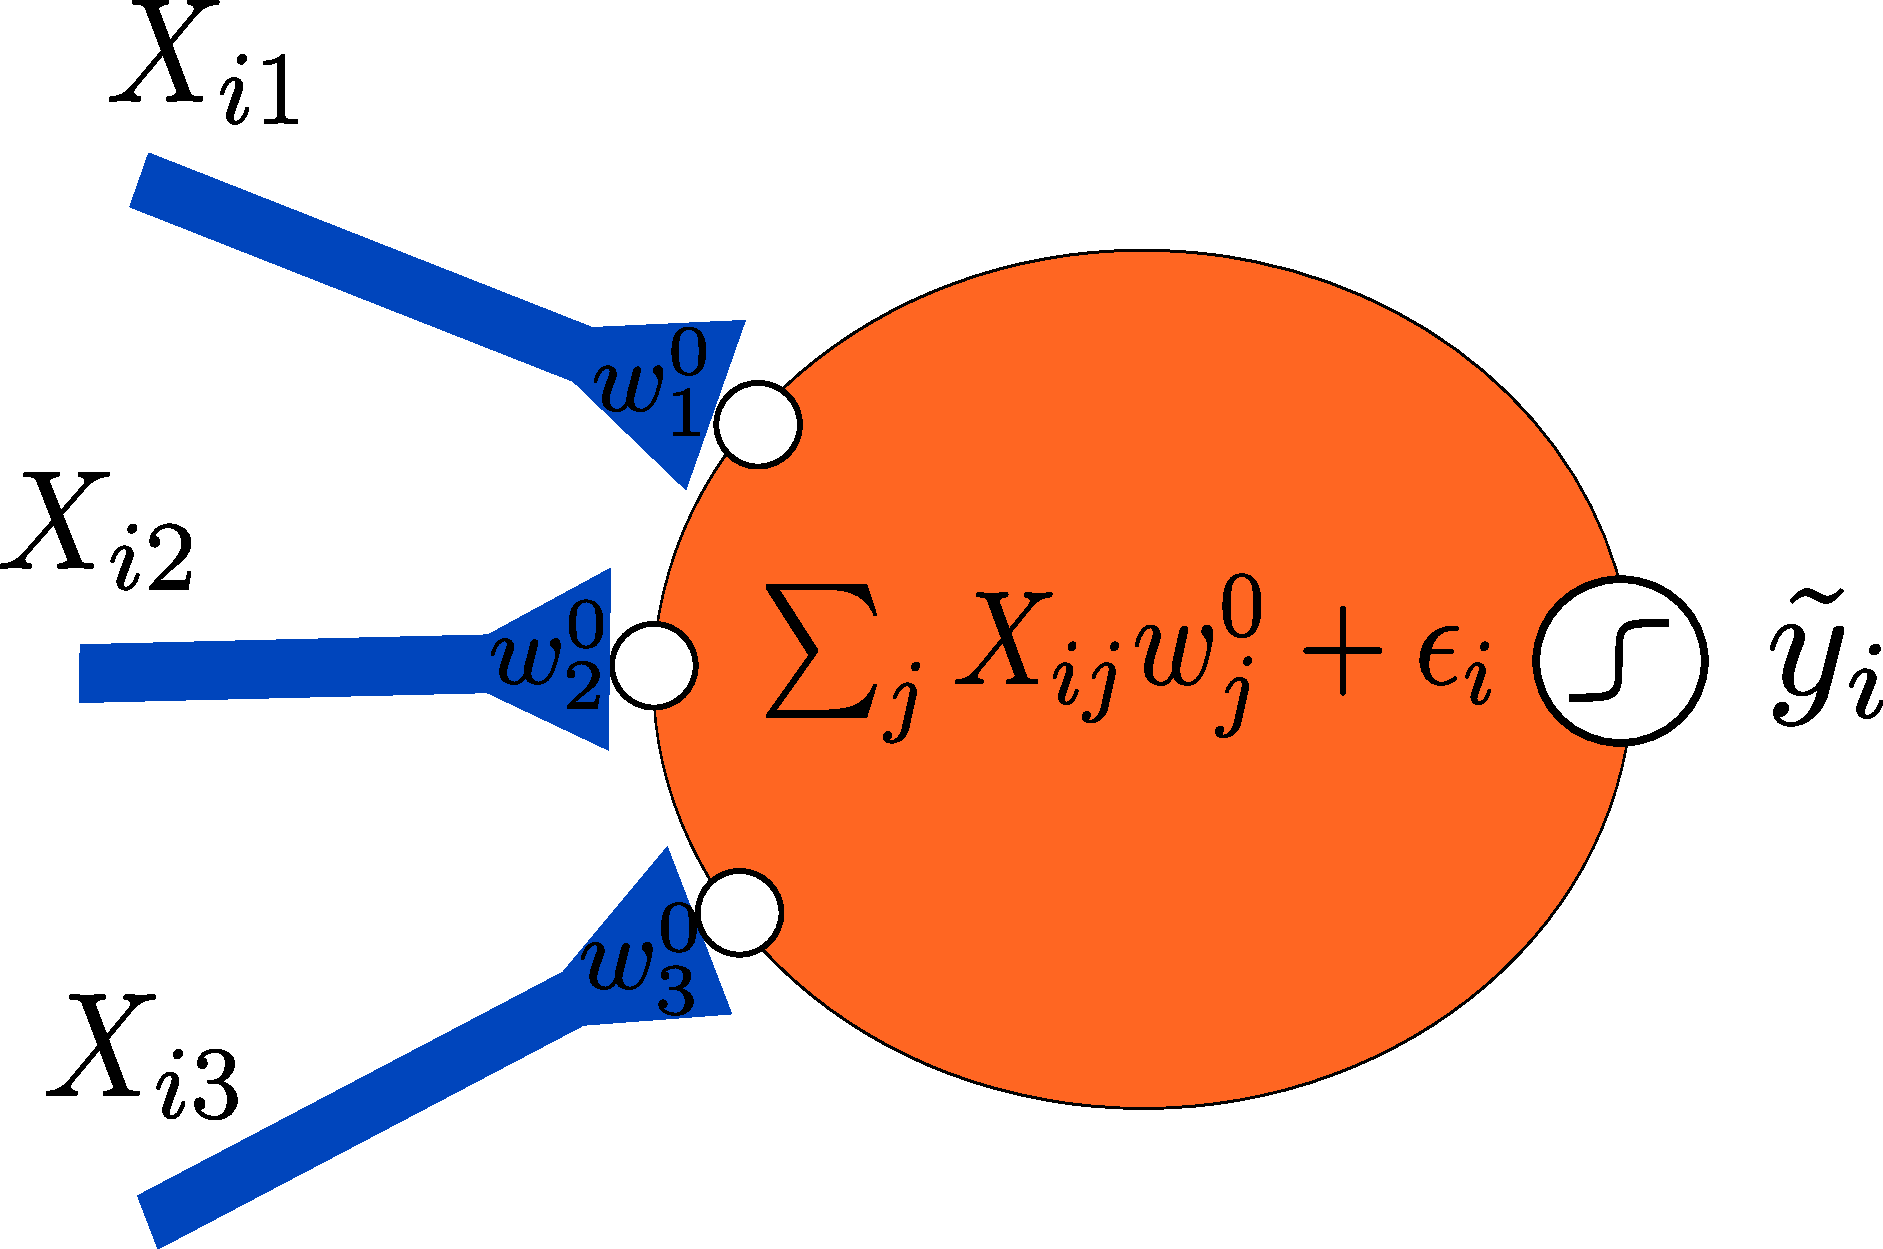
\includegraphics[width = .2\linewidth]{neuronInference.pdf}
\end{flushright}


$y_i = \mathbf{X_i}\cdot \mathbf{w^0} + \epsilon_i \quad \quad i\in [1,\dots N]$

\begin{itemize}
%\item Consider Statistical inference with $N$ data points and $P$ unknowns (predictors).


\item Noise $\epsilon_i \sim f$ not necessarily gaussian

\item (Easy) Classical Regime: $\kappa = P/N\ra 0$
\item (Hard) High Dimensional Regime: $\kappa = P/N \ne 0$

\end{itemize}
\vspace{.2in}



\vspace{.2in}

We want to find $\mathbf{w^0}$


\begin{equation*}
\mathbf{\hat{w}}=\arg \min_{\mathbf{w}}{\left[ \sum_{i} {\rho\left( y_i - \mathbf{X}_{i} \cdot \mathbf{w}\right)}\right]}
\end{equation*}

E.g. $\rho(x) = x^2,|x|,-\log f(x)$

\end{frame}
%-----------------------------


%----------------Frame-------------------
\begin{frame}{Maximum Likelihood}


$P$ fixed, $N\ra \infty$

\begin{equation*}
||\hat{w}-w^0||^2 = \frac{\left(\int{\psi(x)f(x)dx}\right)^2}{\int{\psi^2f(x)dx}}
\end{equation*}

$\psi = \frac{\partial}{\partial w} \rho$

\vspace{.2in}
We find that $\rho_{\text{opt}} = -\log f$


\begin{equation*}
\mathbf{\hat{w}}_{\text{ML}}=\arg\max_{\mathbf{w^0}}{P\left(\mathbf{y},\mathbf{X}|\mathbf{w^0}\right)} =\arg \min_{\mathbf{w}}{\left[ \sum_{i} {-\log f\left( y_i - \mathbf{X}_{i} \cdot \mathbf{w}\right)}\right]}
\end{equation*}





\end{frame}
%----------------------------------










%-----------------Frame-------------
\begin{frame}[t]{Classical vs High Dimensional Optimal M-estimation}

%\note{Fisher information for convolved distribution}

    \begin{block}{Classical}
        \begin{itemize}
        \item $N\ra \infty$, $P/N =\kappa \ra 0$
        \vspace{.1in}
        \item $\rho_{\text{opt}} = -\log f$
        \vspace{.1in}
        \item $\qav{(\hat{w}_i-w^0_i)^2} \ge \frac{\kappa}{\int{\frac{f'^2}{f}}}$
        \vspace{.1in}
        \end{itemize}

    %\begin{flushright} $\epsilon_a \sim f$ \end{flushright}
    \end{block}


    \begin{block}{High Dimensional}
        \begin{itemize}
        \item $N,P\ra \infty$, $P/N =\kappa \in [0,1]$
        \vspace{.1in}
        \item $\rho_{\text{opt}}(x) = -\inf_y{\left[\ln(\zeta(y))+\frac{(x-y)^2}{2 \hat{q}_0}\right]} \quad \quad \quad \quad \zeta = f*\phi_{\hat{q}_0}$
        \vspace{.1in}
        \item $\qav{(\hat{w}_i-w^0_i)^2} \ge \frac{\kappa}{\int{\frac{\zeta'^2}{\zeta}}}$
        \vspace{.1in}
        \end{itemize}
    \end{block}
\end{frame}
%------------------------------------





%-----------Slide-----------------------------------
\begin{frame}[t]{Adding a Regularizer}
    \note{Maximum Likelihood is based on finding the mode of data given the coefficients. Especially in the high dimensional regime, where a prior can really help us, we want to find the mode of the coefficients given the data!}

    \begin{equation*}
        P(\mathbf{w^0}|\mathbf{X},\mathbf{y}) = \frac{P(\mathbf{X},\mathbf{y}|\mathbf{w^0})P(\mathbf{w^0})}{P(\mathbf{X},\mathbf{y})}\propto f(y-\mathbf{X}\cdot \mathbf{w^0})g(w^0)
    \end{equation*}
    
    $w^0_j \sim g$

    \begin{block}{Maximum a Priori}
        \begin{equation*}
            \small{\mathbf{\hat{w}_{\text{MAP}}} =\arg\min_{\mathbf{w}}{\left[\sum_i{-\log f(y_i - \mathbf{X}_i\cdot \mathbf{w})} +\sum_j{-\log{g(w_j)}}\right]}}
        \end{equation*}
    \end{block}

    \begin{block}{Regularized M-estimation}
    \begin{equation*}
        \mathbf{\hat{w}}=\arg \min_{\mathbf{w}}{\left[ \sum_{i} {\rho\left( y_i - \mathbf{X}_{i} \cdot \mathbf{w}\right)} + \sum_j{\sigma(w_j)}\right]}
    \end{equation*}
    Note separability. Solvable for convex $\sigma,\rho$
    \end{block}

\end{frame}
%------------------------------------



%-------------Frame--------------------
\begin{frame}{Motivation}

\begin{equation*}
            \mathbf{\hat{w}} = \arg\min_\mathbf{w} {\sum_a{\rho(y_a - \mathbf{X_a} \cdot\mathbf{ w})} + \sum_i{\sigma(w_i)}}
\end{equation*}
\vspace{.1in}

\begin{block}{Applications}
\begin{itemize}
\vspace{.1in}
 \item{Maximum Likelihood (ML) and MAP commonly applied to High Dimensional Bio-informatics problems, where we should expect poor performance}
     \vspace{.1in}
 \item{Deriving/Understanding the Optimal M-estimator has potential applications for statistical inference and signal processing.}
     \vspace{.1in}
 \item{ Tractability of this form of optimization popular: Compressed Sensing, LASSO, Elastic Net}
\end{itemize}
\end{block}


%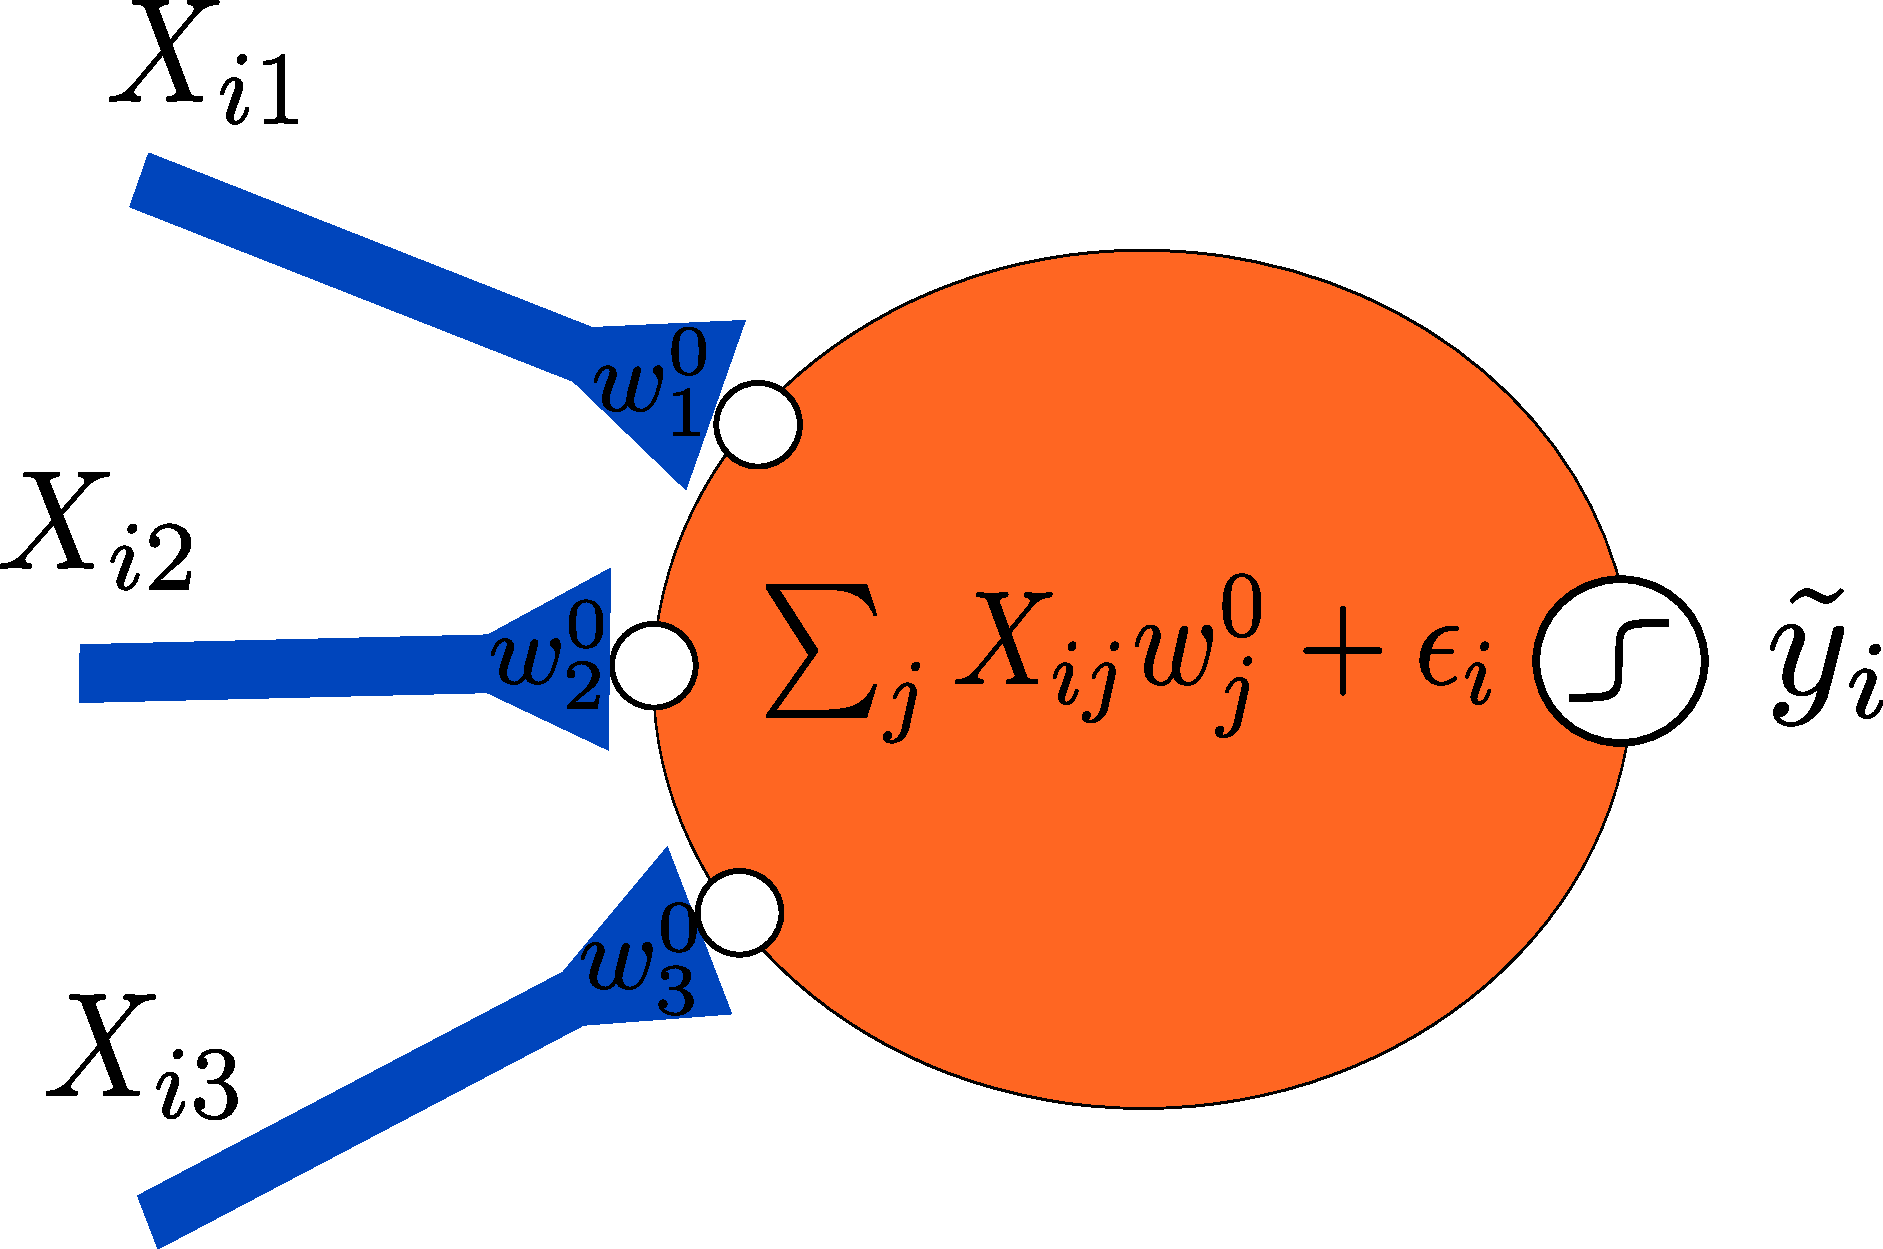
\includegraphics[width = .4\linewidth]{neuronInference.pdf}

\end{frame}
%----------------------------------------


%------------------------Frame------------
\begin{frame}[t]{Statistical Physics Formulation}
Define a spin glass system to solve M-estimator inference

\begin{block}{Spin Glass System}
Define continuous spins $\mathbf{u}=\mathbf{w^0}-\mathbf{w}$. Let the Energy of the system be a function of these spins

\begin{equation*}
 E_{\boldsymbol{\Lambda}}(\mathbf{u})=\sum_i{\rho\left(\mathbf{X}_{i}\cdot \mathbf{u} +\epsilon_i\right)}+\sum_a{\sigma(w^0_a-u_a)}
\end{equation*}

This in turn induces an equilibrium probability distribution on the state

\begin{align*}
P_{G}(\mathbf{u}) &= \frac{e^{-\beta E_{\boldsymbol{\Lambda}}(\mathbf{u})}}{Z_{\boldsymbol{\Lambda}}} & Z_{\boldsymbol{\Lambda}} &= \int{e^{-\beta E_{\boldsymbol{\Lambda}} (\mathbf{u}) }du}
\end{align*}

\begin{equation*}
\lim_{\beta \rightarrow \infty} P_{G}(\mathbf{u}) = \delta\left(\mathbf{u} - \mathbf{w^0} +\mathbf{\hat{w}}\right)
\end{equation*}

\end{block}


\end{frame}
%------------------------------------


%------------Slide---------
\begin{frame}{The Unregularized Case}


\note{Sort of just flashing the form of the solution for the unregularized case.

Falls out quite naturally from replica theory.


Order parameters are important because $q_0$ is the average variance in each error spin.}

\begin{block}{\begin{center}Coupled Equations Relating Order Parameters $q,c$ \end{center}}
\begin{equation*}
\qav{\left(\prox_{c\rho}{(\sqrt{q} z + \epsilon)} -\sqrt{q}z -\epsilon\right)^2}_{z,\epsilon}= \kappa q
\end{equation*}


\begin{equation*}
\qav{\prox_{c\rho}'(\sqrt{q}z + \epsilon)}_{z, \epsilon} = 1-\kappa
\end{equation*}
\end{block}

\vspace{.1in}

\begin{itemize}
    \item $X_{ij}\in \mathcal{N}(0,1/P)$
    \item $\rho$ convex
    \item $\epsilon_i\sim f$ iid
\end{itemize}

\end{frame}
%------------------------------



%--------------Slide------------------
\begin{frame}{Proximal Map}


\begin{block}{Definition}
\begin{equation*}
prox_f(x) = \arg\min_y \left[\frac{(x-y)^2}{2} + f(y)\right]
\end{equation*}

\begin{equation*}
= \left[I + \partial f\right]^{-1} (x)
\end{equation*}


\end{block}
\vspace{.05 in}
Example:
\parbox{.5\linewidth}{
\begin{center}
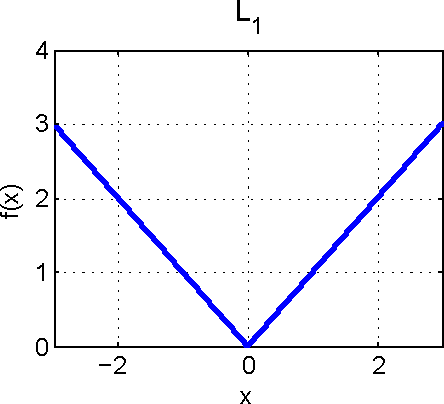
\includegraphics[width = .65\linewidth]{L1_redo.pdf}
\end{center}
}\parbox{.65\linewidth}{
\begin{center}
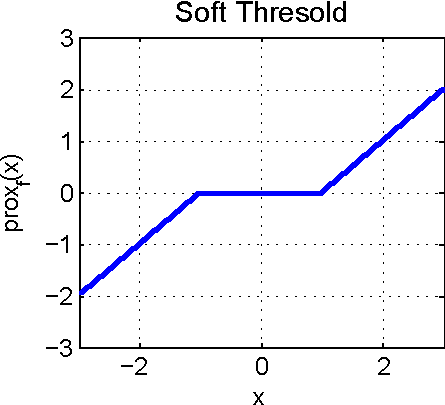
\includegraphics[width = .5\linewidth]{softThresold_redo.pdf}
\end{center}
}


\note{ both $f$ and $\prox_f$ are functions,Known for many functions: e.g. soft thresholding operator for L1 norm. Used in proximal algorithms: minima of $f  \Leftrightarrow$ fixed points $ prox_f$}


\end{frame}
%----------------------------------------








%\parbox{.40\textwidth}{
%\begin{block}{Order Parameters}
%$q =$
%$c =$
%\end{block}
%}\parbox{.38\textwidth}{
%\begin{center}	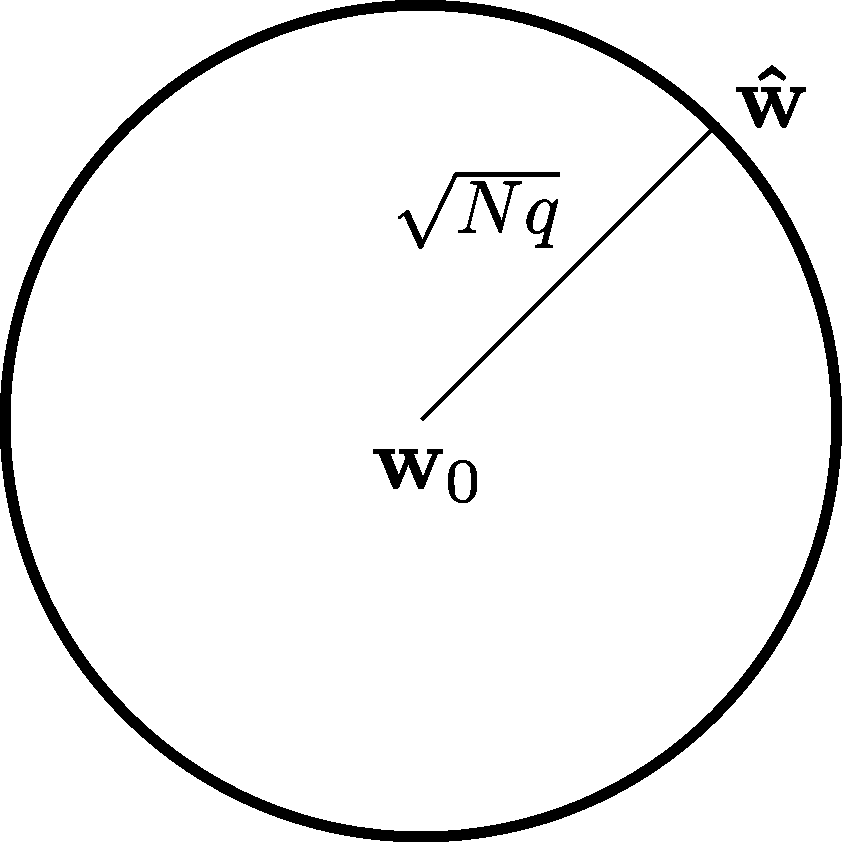
\includegraphics[width=0.5in]{errorCircle.pdf}
%\end{center}
%}

%\parbox{.45\textwidth}{
%\begin{center} 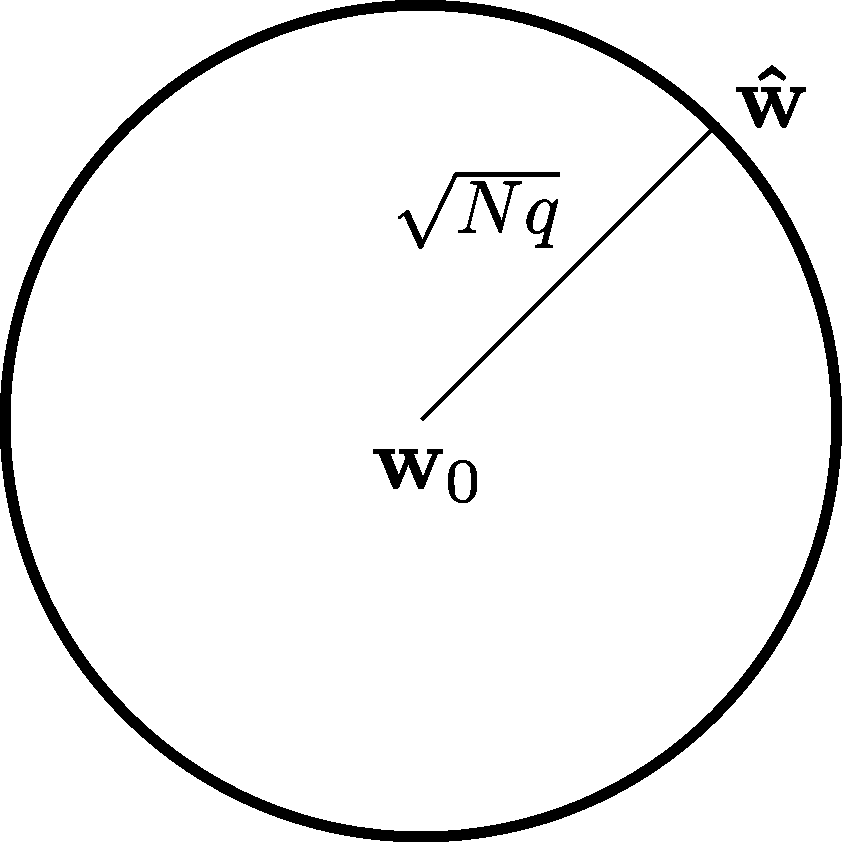
\includegraphics[width=0.4\linewidth]{errorCircle.pdf}
%\end{center}
%}


%
%-------------Slide---------------
\begin{frame}{Analytic Estimator Error}
How to choose $\rho$ to minimize $q$?

    \begin{center}
        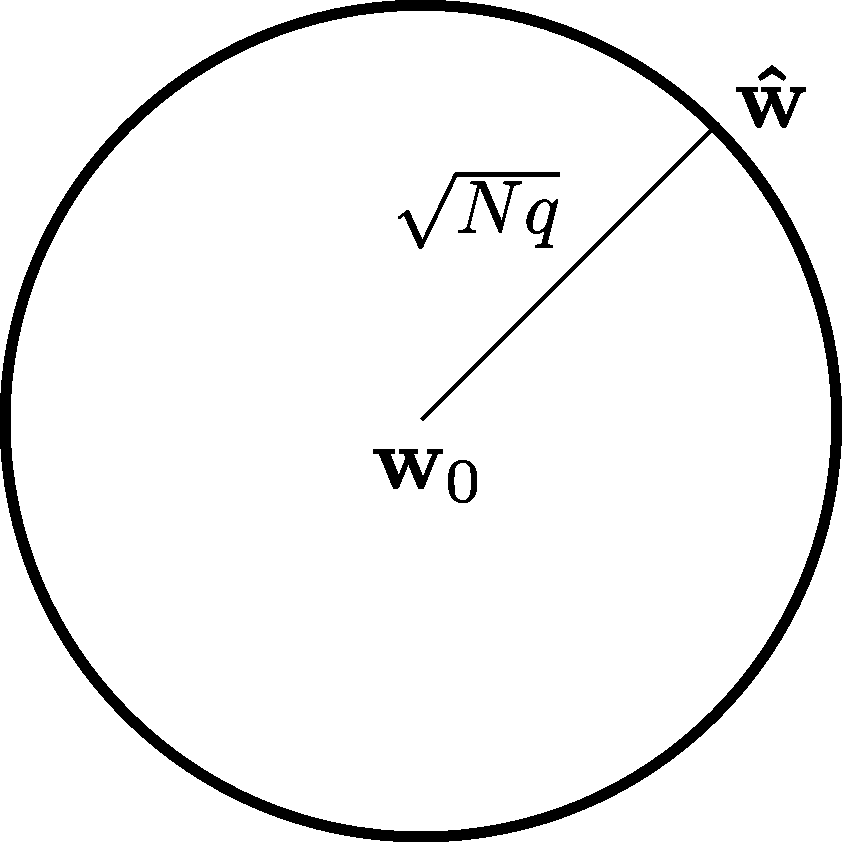
\includegraphics[width = .3\linewidth]{errorCircle.pdf}
    \end{center}


    \begin{equation*}
    \qav{\left(\prox_{c\rho}{(\sqrt{q} z + \epsilon)} -\sqrt{q}z -\epsilon\right)^2}_{z,\epsilon}= \kappa q
    \end{equation*}

    \begin{equation*}
    \qav{\prox_{c\rho}'(\sqrt{q}z + \epsilon)}_{z, \epsilon} = 1-\kappa
    \end{equation*}
\end{frame}
%----------------------------------------




%-----------Slide-----------------------------------
\begin{frame}[t]{Optimal Unregularized M-estimator}



    \vspace{.2in}

    \begin{block}{Optimal M-estimator}
        \begin{align*}
            \rho_{\text{opt}}(x) &= -\inf_y{\left[\ln(\zeta_{\hat{q}}(y))+\frac{(x-y)^2}{2 \hat{q}}\right]} & \zeta_{\hat{q}} &= f*\phi_{\hat{q}}
        \end{align*}
        \begin{align*}
           \hat{q} = \min{q} \quad \quad \text{s.t.} \quad q I_{q} &=\kappa & I_{q} = \int_{-\infty}^{\infty}{\frac{\zeta_{q}'^2(y)}{\zeta_{q}(y)}dy}
        \end{align*}


        \begin{itemize}
        \vspace{.1in}
        \item $\hat{q}$ - best possible asymptotic MSE for a convex M-estimator

        \item $\rho_{\text{opt}}$ is the optimal loss function (assuming log-concave noise)

        \item{Note: Not maximum likelihood, and $\rho$ varies with dimensionality $\kappa$}
        \end{itemize}

    \end{block}

\end{frame}
%------------------------------------





%--------------------Frame-----------------------
\begin{frame}{Optimal Unregularized M-estimator}


        \begin{center}
            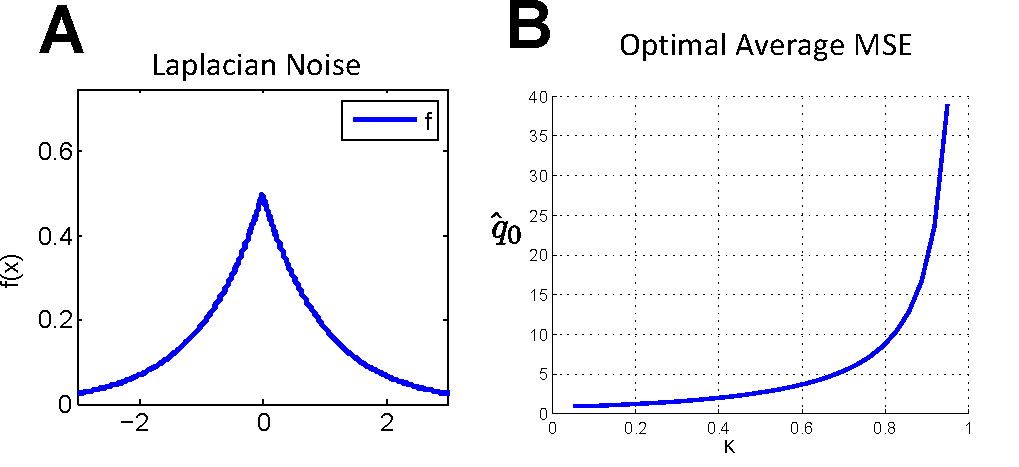
\includegraphics[width = .5\linewidth]{unRegNoiseOpt.pdf}
        \end{center}


        \begin{center}
            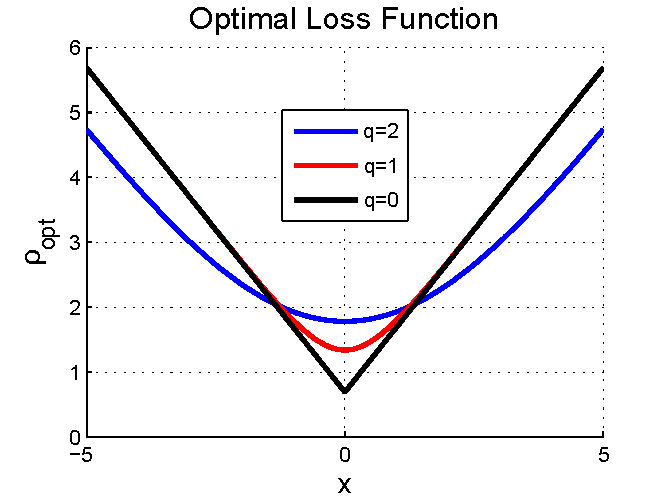
\includegraphics[width = .5\linewidth]{opt_loss.pdf}
        \end{center}

\end{frame}
%------------------------------------------------


%-------------------Frame---------------------
\begin{frame}[t]{Regularized M-estimation}
\note{Again we ask the same question, which M-estimator (strategy) minimizes q? Obviously it will depend on the distribution of noise and coefficients, in the next slide I'll show how.}
\begin{equation*}
y_i = \mathbf{X}_i \cdot \mathbf{w^0} + \epsilon_i \quad \quad \quad \quad \quad w_j^0\sim g, \epsilon_i \sim f
\end{equation*}

\vspace{.3in}
\begin{equation*}
            \mathbf{\hat{w}} = \arg\min_\mathbf{w} {\sum_a{\rho(y_a - \mathbf{X_a} \cdot\mathbf{ w})} + \sum_i{\sigma(w_i)}}
\end{equation*}

\vspace{.2in}
\begin{center}
        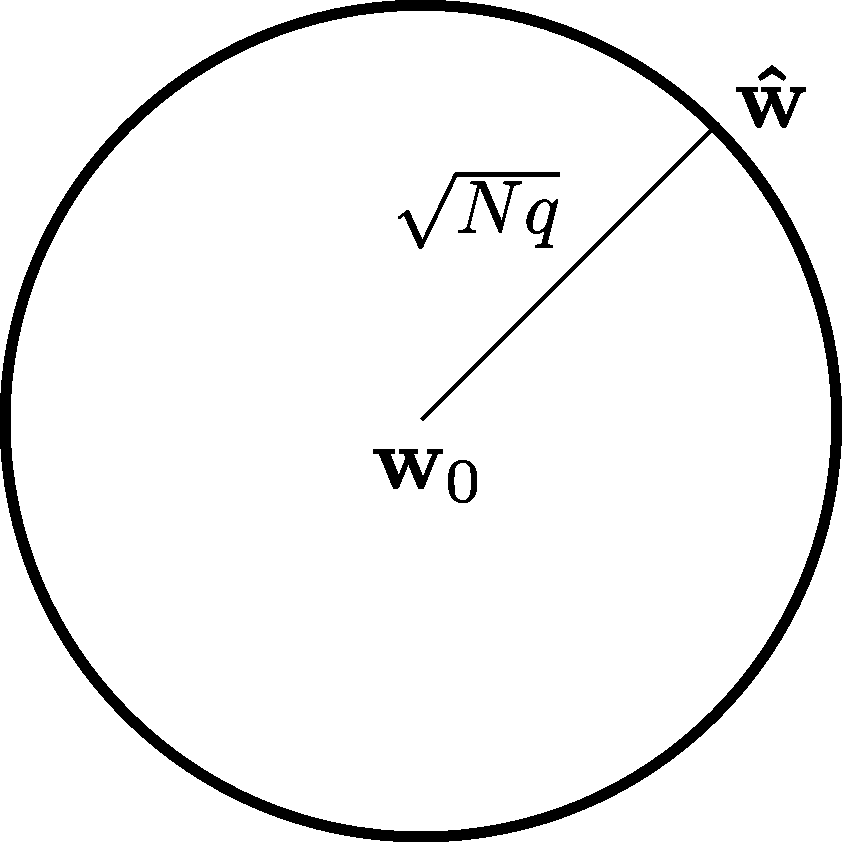
\includegraphics[width = .25\linewidth]{errorCircle.pdf}
\end{center}




\end{frame}
%---------------------------------------------





%------------------------Frame-------------------
\begin{frame}{Regularized M-estimation}
\note{We know we can do better if we have some prior on our signal, and in the regularized case we can again work out the replica solution}

\begin{block}{Optimal Inference}
\begin{equation*}
 \rho_{\text{opt}}^R(x) =  -\inf_y{\left[ \ln(\zeta_{\tilde{q}_0}(y)) + \frac{(x-y)^2}{2 \tilde{q}_0}\right]}
\end{equation*}
\begin{equation*}
\sigma_{\text{opt}}^{R}(x)=-\frac{\tilde{q}_0}{\tilde{a}}\inf_y{\left[ \ln(\xi_{\tilde{a}}(y)) +\frac{(x-y)^2}{2 \tilde{a}}\right]} \label{optReg}
\end{equation*}

%\begin{equation}
%\begin{split}
%\rho_{\text{opt}}^R(x) &= -\inf_y{\left[ \ln(\zeta_{\tilde{q}_0}(y)) + \frac{(x-y)^2}{2 \tilde{q}_0}\right]} \\
%\sigma_{\text{opt}}^{R}(x) &= -\frac{\tilde{q}_0}{\tilde{a}}\inf_y{\left[ \ln(\xi_{\tilde{a}}(y)) +\frac{(x-y)^2}{2 \tilde{a}}\right]}\\
%\label{nbOpt}
%\end{split}
%\end{equation}


\begin{equation*}
\begin{split}
\tilde{q}_0,\tilde{a} &= \arg\min_{q_0,a}{q_0} \\
\text{s.t. }\quad  a I_{q_0} & = \kappa,\quad a^2 J_a = a-q_0
\label{unregopt}
\end{split}
\end{equation*}


\begin{itemize}
\item $\rho_{\text{opt}},\sigma_{\text{opt}}$ are optimal M-estimator (log concave $f,g$)

\item $\tilde{q}_0$ is the asymptotic MSE
\item $\tilde{q}_0,\tilde{a}$ are smoothing parameters
\end{itemize}
\end{block}
\end{frame}
%--------------------------------------------------




%--------------------Frame-----------------------
\begin{frame}{Unregularized M-estimator}


        \begin{center}
            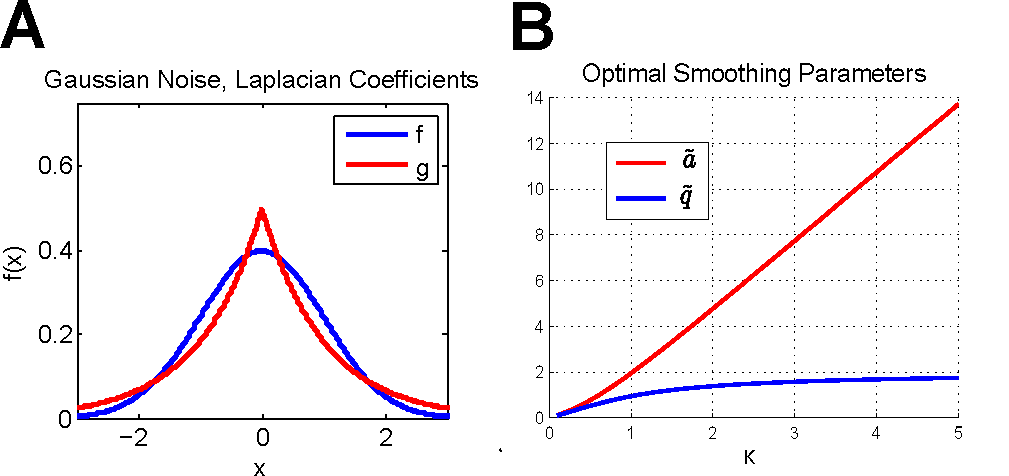
\includegraphics[width = .7\linewidth]{regularizedPlots.pdf}
        \end{center}


\end{frame}
%------------------------------------------------


%--------------------Frame-----------------------
\begin{frame}{M-estimator Comparison}


\begin{center}
    $\rho_{\text{MAP}}(x) = \frac{x^2}{2} \quad\quad \sigma_{\text{MAP}}(x) = |x|$

    $ \rho_{\text{Ridge}}(x) = \frac{x^2}{2} \quad\quad \sigma_{\text{Ridge}}(x) = \frac{x^2}{2}$
\end{center}


\vspace{.1in}
        \begin{center}
            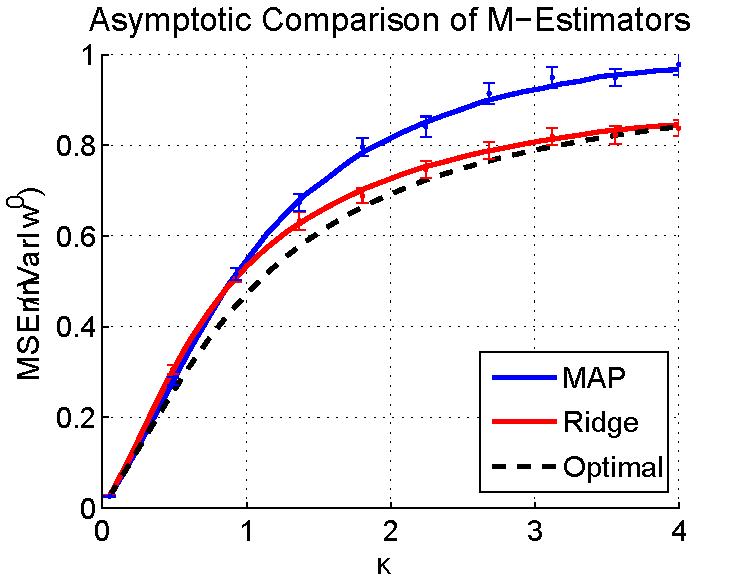
\includegraphics[width = .55\linewidth]{CompareM_est_redo.pdf}
        \end{center}
\end{frame}
%------------------------------------------------




%---------------------Slide----------------
\begin{frame}{Future Directions- LN models}

$y_i = \eta(X_i \cdot w^0) + \epsilon_i$


\end{frame}
%-----------------------------------------


%---------------------Slide----------------
\begin{frame}{Future Directions - Random Dimensionality Reduction}




\end{frame}
%-----------------------------------------


%---------------------Slide----------------
\begin{frame}{Future Directions - Phase Transitions in Clustering}




\end{frame}
%-----------------------------------------



%---------------------Slide----------------
\begin{frame}{Future Directions - Phase Transitions in Clustering}
\end{frame}
%-----------------------------------------

















\end{document} 